\chapter{Introduction}
\section{Background}
\label{background}
Electricity distribution networks, and the way in which they are managed, are currently going through a significant transition, with perhaps more change over the last ten years than in the previous hundred. %the sort of statement where a ref would help strengthen it, but OK not to have
Until recently, generation and load were largely viewed and managed separately: power was produced almost exclusively by large, centralised generating units, and was consumed by customers after routing via %traversing is not quite right word. reticulation... hmm???
the transmission and distribution networks. 
Networks were designed and built for demand profiles which were relatively stable over time, with demand forecasting at distribution feeder level required primarily for long term network planning purposes only. 
Increasingly, power is both consumed by customers connected to the distribution network and is also generated and manipulated by distributed energy resources (DER) within the distribution network, often behind the meter of individual consumers. 
The impact of increasing levels of DER in the system creates, among other things, both a need and an opportunity to more actively manage distribution networks, while also resulting in a generally less predictable net demand profile.

DERs are controllable devices in the power network that generate, store, and/or consume power. 
This includes solar photovoltaic generation (PV), battery storage, and electrical vehicles. 
In Australia, the dominant DER technology deployed to date is solar PV, with over 1.8 million systems now reportedly installed on residential properties \cite{apvi2017}. 
It is widely anticipated that battery storage and electrical vehicle uptake may be just as rapid \cite{bloomberg2018}.

The Tasmanian distribution network, meanwhile, is forecast to experience significant increases in these technologies by 2025: \\
\begin{itemize}
	\item 680\% increase in battery storage capacity (from 11MWh to 75MWh) \cite{Jacobs2017}
	\item 170\% increase in PV installation capacity (from 130MW to 220MW) \cite{Jacobs2017}
	\item 39\% of new car sales will be electrical vehicles - the highest in the country \cite{AEMO2016}
\end{itemize}

The changing nature of the distribution network presents an opportunity to maximize the use of existing assets by delaying the need for network augmentations, while also providing customers with a more reliable supply of power.
For example, batteries could be used to peak-shift, reducing maximum feeder load.
However, to achieve this reliably and with optimal use of available DER generally requires sophisticated methods to optimize the power flow to and from the distributed resources.

\begin{figure}[htbp]
	\centerline{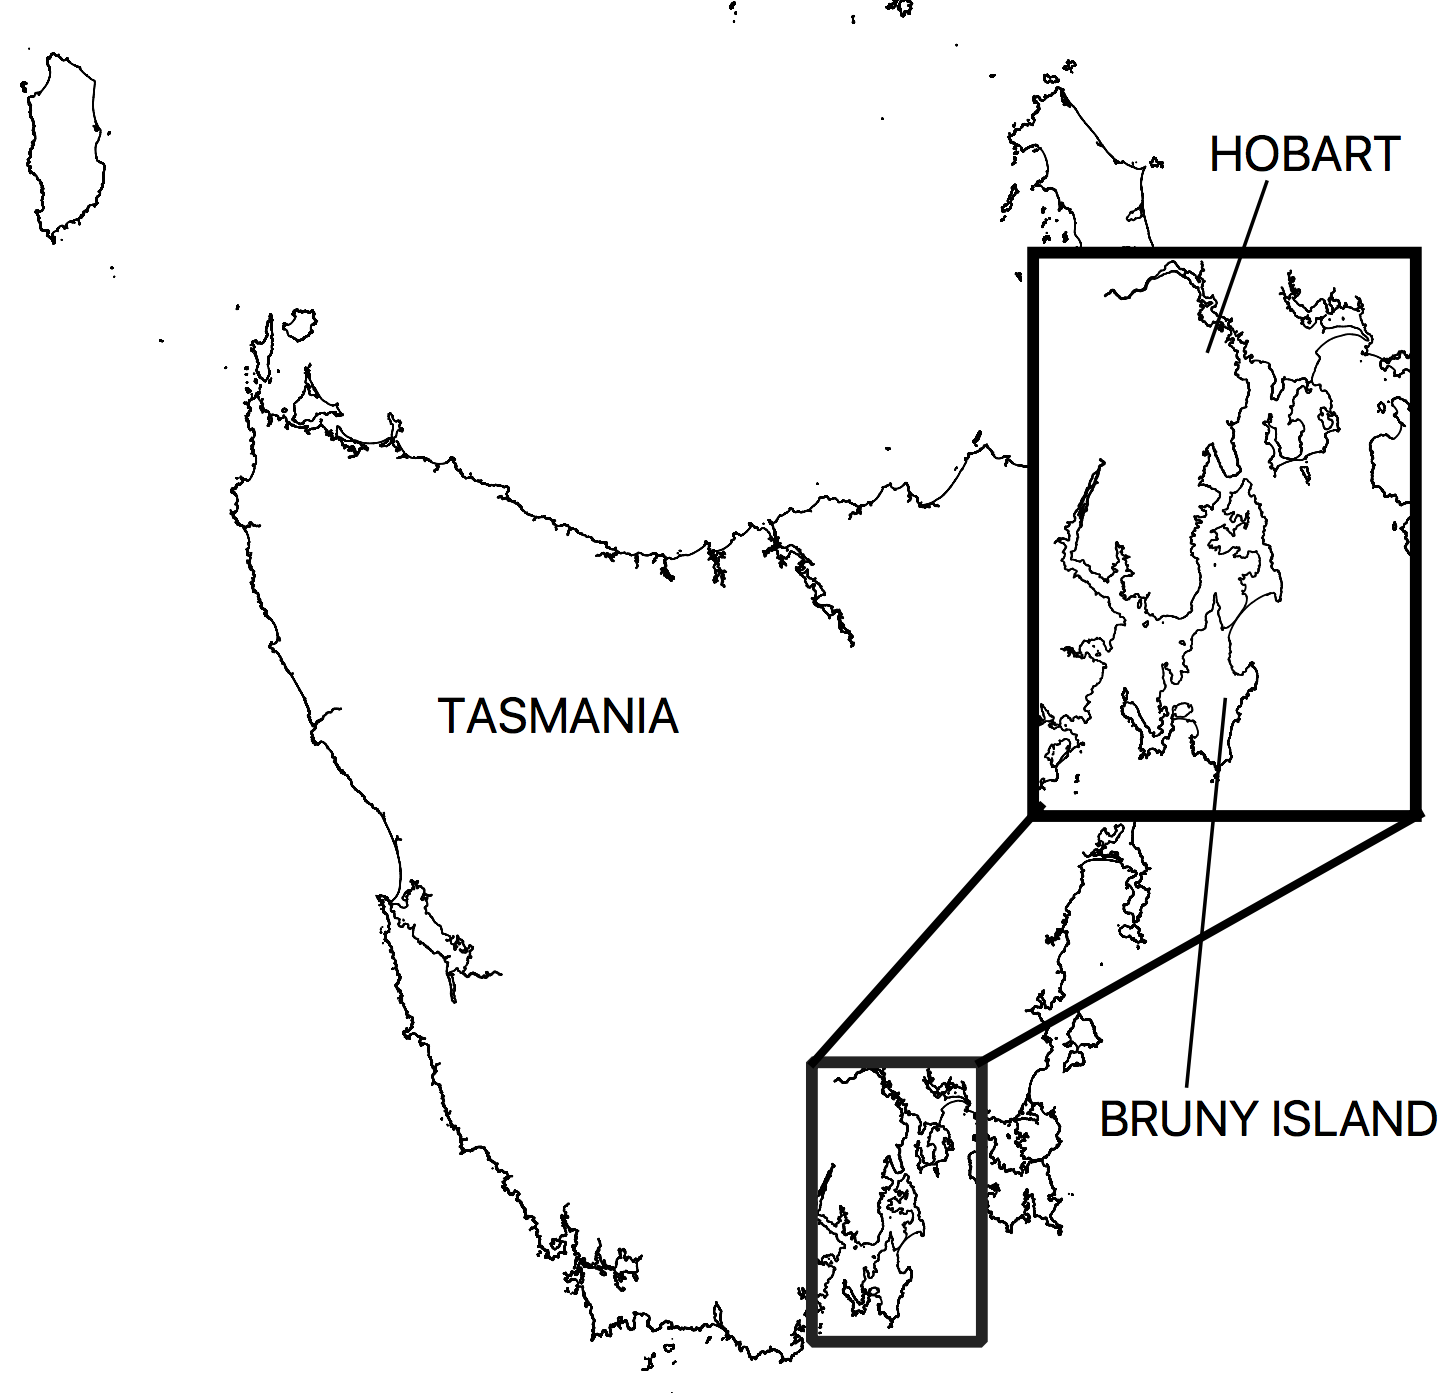
\includegraphics[width=.5\textwidth]{images/bruny_island_map.png}}
	\caption{Bruny Island in southeast Tasmania experiences significant increases in load during holiday periods and was used as a case study for the load forecaster.}
	\label{fig:bruny_map}
\end{figure}

One method to achieve this coordination of DER in distribution networks is presented in \cite{Scott2014} and has been implemented on Bruny Island, Tasmania as part of the CONSORT project (CONSumer energy systems providing cost-effective grid suppORT).
Bruny Island, shown in Figure \ref{fig:bruny_map}, is a popular holiday destination and during peak periods --- such as Easter morning and afternoon peaks --- the submarine feeder supplying the island becomes overloaded and is supplemented by a diesel generator located on the island.
The aim of the CONSORT project was to effectively peak shift the load away from the morning and afternoon peaks to prevent the use of the generator.

To fulfil such an objective while using the available distributed resources optimally, the CONSORT project relies upon having an accurate, online, 24-hour horizon forecast at the feeder level.
However, load forecasting methods commonly employed in industry are neither intended to forecast with high accuracy over a time period this short nor at the feeder level. \cite{CIGRE2016}.
An improved method for producing accurate feeder-level forecasts is not only highly desirable for this project, but will also in the future become a critical element of active distribution network management more generally.

In this thesis, a novel neural network-based day-ahead feeder level load forecasting system is developed, with its performance evaluated using ten years of historical demand data for training and testing. The forecaster is implemented live on Tasmania's Bruny Island distribution network, enabling the CONSORT project's residential battery systems to effectively support the network during periods of peak demand.

\section{State of the art in load forecasting}

\subsection{Load forecasting - definition and general remarks}
Before looking at state of the art load forecasting methods, it is important to first establish precisely what load forecasting is.
Load forecasting is the process of predicting the electricity demand in a particular area at each period over a planning horizon \citep{Weron2006}.
For example, a load forecast with a period (or resolution) of one hour and a horizon of 24 hours would forecast the load at each hour over the next 24 hours.
It is a specific case of time series forecasting.
Load forecasting can be broadly categorised into short-term (STLF), medium-term (MTLF), and long-term load forecasting (LTLF).
The exact horizon for each category differs between publications, but it is widely accepted that anything with a forecast horizon of up to 24 hours is short-term load forecasting.
This thesis will deal exclusively with STLF.
Generally load forecasting systems uses exogenous information as input, such as weather and date information, along with historical load data in order to produce a forecast.

What is clear throughout the literature is that there are a handful, perhaps a dozen or so, of clearly distinct techniques that are commonly applied to load forecasting.
However, these methods are nearly always mixed, matched, and combined to form a complete forecasting system.
As a result, there are a combinatorial number of approaches to forming a load forecasting system.
This section will attempt to cover only the most prolific techniques, and the examples cited will generally also employ techniques which have not been discussed.

The literature presents no single load forecasting system that is superior under all conditions.
A system that is well suited to forecasting load with a majority industrial customers may be poorly suited to forecasting load with a majority residential customers.
This is because there is no single load forecasting problem - every household, feeder, and power system exhibits different patterns as a result of the different customers attached to it and thus presents a different problem.
As a result, it is invalid to compare the performance of forecasting systems unless they are evaluated on the same datasets, making it difficult to establish a state of the art approach even at a similar aggregate level of load.

\subsection{Load forecasting in industry}
In section \ref{background} it was stated that load forecasting methods commonly employed in industry neither intended to forecast with high accuracy over a 24 hour period nor at feeder level in the distribution network.
This is supported by a survey conducted by CIGRE in 2016 \citep{CIGRE2016} showing that, of 29 utilities, 79\% use load forecasting for long term planning and 32\% for short term operational planning.
Interestingly, this survey also found that the majority of load forecasting software is developed in-house, and the methodology used is usually revised at least every four years.

The lack of attention to load forecasting at the feeder level is certainly echoed in the literature.
The vast majority of published work considers forecasting at the city level and above, with a smaller portion looking at sub-GW load, and an even smaller portion looking at sub-MW load.
Additionally, the publications looking at lower levels of aggregate load tend to be more recent, and are predominately published as conference papers rather than in peer-reviewed journals.

\subsection{Patterns in load profiles}
\label{patterns-profiles}
In a residential setting, such as a residential feeder, power is consumed as a result of customer actions - taking a shower causes the hot water system to consume power to reheat water, turning on a kettle or toaster causes power to be consumed, use of air conditioning results in power consumption, etc.
It is intuitive to expect that there would be patterns underlying these actions or behaviours; customers probably take showers more often in the morning, and when it is cold customers are probably more likely to turn on their heaters.
If the feeder in question happens to be in a popular holiday destination, then it might also be the case that overall more power is consumed during holiday periods as a result of more customers being in the area.
Conversely, a feeder in a commercial area may experience a reduction in load over holiday periods because the workers are away.
Any load forecasting system must be able to intrinsically model these underlying patterns if it is to effectively predict load.

Before looking at load forecasting techniques and systems, the typical patterns of load profiles will be discussed.
It must be kept in mind though that all conclusions presented here are general; they will likely vary between countries, cultures, and feeders.
Analysis of a specific feeder is undertaken in section \ref{bruny-data-analysis}.

\subsubsection{Calendar day}
The most significant factor contributing to a load profile is the calendar day \citep{Weron2006}.
Generally weekdays and weekends have differing load profiles, and even days during the week can be observed to have significantly different profiles.
Meteorological seasonality usually plays a large role in load variation over a full year.
This may be a direct result of day of the year, such as in the case of a commercial load that only operates over summer, or it may actually be a result of weather.
Finally, holiday periods cause large deviations from standard profiles and can be difficult to predict due to the relatively few examples available.
Holidays can also affect days adjacent to them as people may also take these days off work.

\subsubsection{Weather}
Second to calendar day, the most significant factor behind the load profile is weather \citep{Hippert2001}.
Typically temperature and humidity are considered the most influential, as they drive customers to use heating and cooling which both consume large amounts of power.
More recently, cloud cover and solar irradiance have become increasingly important as they affect rooftop photovoltaic (PV) generation \cite{AEMO2017}.
In regards to PV, it may be further necessary to model its uptake - solar capacity is increasing in Australia \citep{Jacobs2017} and so a forecasting system that relies on past examples to create future predictions may need to account for this.

\subsection{Similar day and clustering}
As load profiles are dependent primarily on calendar day and weather, a rudimentary load forecasting system can be implemented by simply finding a load profile from the past that has the most similar calendar day and weather properties to the period being forecast. 
Similarly, a clustering approach can be taken if it is assumed that load profiles will repeat themselves as a result of repeating weather and calendar day patterns.

\citet{Rahman1993} used an expert-system based method to select a set of similar days from the past. 
These days were then modified by use of a lookup table based on differences in temperature and other exogenous factors between the similar and forecast period.
Finally, all similar days were regressed to form a forecast.
This method achieved a mean absolute percentage error (MAPE) of around 2\% when forecasting at the level of a a single state of the United States with a 24-hour horizon.

\citet{Senjyu1998} used a weighted sum-squared-error between the maximum temperature, minimum temperature, and day type of the period being forecast and previous days to select the most similar five days from the past.
A fuzzy logic system was then used to generate weights to augment the similar days based on differences in weather and differences in load profile between the similar day and the day prior to the forecast day.
This was found to out-perform a more rudimentary systems which only used average load of the similar days.
The system achieved a MAPE of around 2.5\% when forecasting hourly load of approximately 600MW with a 24-hour horizon.
Interestingly, this system was further extended \cite{Senjyu2004} to use a recurrent neural network instead of a fuzzy logic system and this resulted in a decrease in MAPE to 2.8\%.

\citet{Dou2018} used K-means clustering combined with variational mode decomposition and a self-adaptive evolutionary extreme learning machine to predict the load demand for renewable generation.
The system assigns historical days to clusters and then finds the most similar cluster to the day being forecast and uses properties from that cluster to produce a forecast.
The system was applied to forecasting photovoltaic power output, wind power output, and electrical load.
The system achieves a mean absolute error of 10.8 MW when forecasting hourly load of around 60 MW with a 24-hour horizon.

\subsection{Autoregressive integrated moving average}
Autoregressive integrated moving average (ARIMA) models, introduced by \citet{Box1970}, are used widely for time series forecasting \citep{Weron2006}. 
Generally, ARIMA models are used at the core of the forecasting system, and other methods are used in a supporting role.
ARIMA-based models are generally considered to be complex and require a great deal of experience to effectively select appropriate parameters \citep{Desouky2000}.

\citet{Taylor2007} applied a seasonal autoregressive moving average (ARMA) model to forecast a variety of European loads, with means of between 3 and 50 GW.
The method achieves an accuracy of approximately 1.75\% when performing hourly forecasts with a 24-hour horizon.
This was extended by \citet{Arora2013} who used a rule-based system combined with the seasonal ARMA model to more accurately predict anomalous holiday periods.
This rule based system dictates the intrayear seasonal cycle of the model, which is set such that it corresponds to both a matching anomalous day (Easter, Christmas, etc.) from a previous year and a matching day of the week from a previous year.
Thus, the model will take historical data from the same anomalous day occurring on the same day of the week at some time in the past.
This rule decreased the MAPE on anomalous days from approximately 5\% to approximately 3\% when evaluated on data from Great Britain with a typical load of around 30 GW.

\citet{Bennett2014} used an ARIMAX model to forecast the properties of the next day's load (next day peak demand, next day morning peak, and next day total energy usage). These properties were then provided to a neural network which selected the appropriate cluster for the day, whose load profile mean was then modified to better match the predicted properties.
The system achieves a MAPE of 12\% when forecasting hourly loads of around 60 kVA over a 7-day horizon.

\citet{Karthika2017} used an ARIMA model to perform a preliminary load forecast, which was then augmented by a support vector machine to account for non-linear exogenous variables such as temperature and day of week.
The method achieved a MAPE of 4.15\% on an hourly 24-hour horizon forecast.

\citet{Amjady2001} used an ARIMA model which was augmented by estimated forecasts from human power system operators.
This additional information allowed the system to achieve a MAPE of approximately 1.75\% when forecasting load on the order of 10 GW with hourly resolution and a 24-hour horizon.
This compares to a MAPE of about 3\% for a standard ARIMA model.
This system has the downside of relying entirely upon a specialist expert to provide regular input information.

\subsection{Support vector regression}
Support vector regression (SVR) was introduced by \citet{Drucker1996} and has been applied widely to short-term load forecasting.
SVR maps an input feature vector into a higher dimensional space and applies linear regression.

\citet{Ceperic2013} applied an ensemble of 24 SVR models to predict each hour of a 24-hour forecast.
This was found to out-perform wavelet transform neural network methods \cite{RochaReis2005}\cite{AMJADY2009}, and echo state neural networks \cite{Deihimi2012}.
The SVR ensemble achieves a MAPE of 1.31\% when forecasting hourly load with a 24-hour horizon on the ISO New England dataset.
This load is on the order of 15 GW.

\citet{Elattar2010} modified SVR such that during the training phase the more recent historical data had a larger influence on the model parameters.
This approach achieved a MAPE of 3.62\% when forecasting hourly load with a horizon between 16 and 88 hours on a dataset with a mean load of around 2.5 GW.


\subsection{Artificial Neural Network}
An artificial neural network (ANN) is a method for computation based loosely on biological brains \citep{negnevitsky2005artificial}.
ANNs can take on widely differing structures, and have have achieved state of the art performance in a wide range of fields including handwriting recognition \citep{2017arXiv171009829S}, machine translation \citep{Vaswani2017}, speech recognition \citep{Chiu2017}, and speech synthesis \citep{DBLP:journals/corr/OordDZSVGKSK16}.
ANNs have been demonstrated to out-perform ARIMA models for electricity time series price forecasting \citep{Mandal2010}.
For short-term time series vehicle traffic forecasting, ANNs have been shown to outperform both ARIMA and SVM (SVR) models \cite{Zhao2017}.

\citet{Chen2010} employed a wavelet neural network and similar day selection to perform a load forecast with a 24-hour horizon and 1-hour resolution.
The load being forecast was on the order of 15 GW (ISO New England dataset) and the forecast was performed only once per day, at 9am.
The authors calculated the wind chill temperature, based on ambient temperature and wind speed, and transformed it to have a linear relationship with load before using it as an input to the system.

\citet{Kong2017}\cite{Kong2018} applied a long short term memory recurrent neural network for short term load forecasting of aggregate household load.
The loads of 69 households were aggregated to form a load time series varying between 0 and 3000 kW.
Forecasting this time series resulted in a MAPE of 8.59\%.
Additionally, the method was used to forecast individual household loads, achieving a MAPE of 44.39\%.
The paper does not state the forecast horizon or resolution.
This method was found to out perform simpler multilayer perceptron models and clustering-only methods.
These results are achieved without the need to perform any data manipulation other than scaling between zero and one and using one-hot encoded data for date and holiday information.
Additionally, the system requires only a single neural network model for forecasting at any time.

\citet{Ding2016} applied a multilayer perceptron neural network to forecasting residential feeder level load with hourly resolution and a 24-hour horizon.
The load was split into daily average power and intra-day load fluctuations, and each was forecast separately.
Interestingly, their justification for use of a multilayer perceptron is that it is a universal function approximator.
While true in theory \cite{Hornik1989MultilayerFN}, this statement pays no regard to the complexity of the neural network nor the methods by which the neural network parameters must be found.
When evaluating the forecaster on a residential feeder with a mean load of around 50 kW a MAPE of 10.3\% and mean absolute error (MAE) of 3.63 kW was achieved.
When evaluating on a commercial feeder the system achieves a MAPE of 15.5\% and a MAE of 75 kW - worse performance than the residential case despite the higher load.
This discrepancy is put down to the residential feeder being the aggregate of many individual small independent customers, while the commercial feeder is an aggregate of only several customers.
By the central limit theorem the residential feeder load at a given instant in time will more closely represent a normal distribution.

\citet{Hernandez2014} applied a multilayer perceptron to forecasting load in the 25 MW range.
Sine and cosine functions were used to encode date information before supplying it to the neural network.
The forecasting system achieves a MAPE of 2.4\% when performing hourly forecasts with a 24-hour horizon.
The paper presents a graph of MAPE versus forecast horizon, and notably the MAPE is not lower earlier in the forecast, as it is in most other papers.

\citet{Sun2016} applied wavelet neural networks to forecast load in a distribution network in a hierarchical fashion.
The substation level load was forecast first, then feeders, transformers, and finally individual customers.
The forecasting system was evaluated on six feeders from the same substation, with mean loads ranging from 2.5 to 8 MW, and achieved MAPE scores between 3.5\% and 5\%.


\section{Problem formation and scope}
\label{scope}
The aim of this thesis is to build upon existing research and develop a load forecasting system which can predict future load based on weather, holiday periods, and other exogenous factors. 
Bruny Island and the CONSORT project will be used as the primary case study. 
The forecasting system is expected to be equally applicable to any feeder or power system.
Specifically, the system will have the following properties:
\begin{itemize}
	\item The forecasting system will be designed to be practical to implement in industry; specifically it should not require specialised skills to operate, and nor should it require significant modifications when forecasting different feeders.
	\item The forecasting system will produce a forecast with a horizon of up to 24 hours in the future in 30- and 60-minute intervals.
	\item The forecast will be able to begin from any point time.
	\item The forecasting system will predict load in kVA at each interval.
	\item The forecasting system will be aimed at predicting aggregate load at the feeder level. That is, between approximately 0.5 and 10MVA.
	\item The forecasting system will be especially aimed at predicting load during anomalous holiday periods.
\end{itemize}
